

\chapter{Concept of our solution} %\label{cha:eva}}
In this chapter we will introduce the initial proposed solution. The dataset, which we use in our work, will be presented with a specific example. Lastly, a plan for the future work will be introduced.
\section{Proposed solution}
As it emerges from our research of the state-of-the-art, standard and the most exploited deep learning approach to classification tasks in medical imaging is undoubtedly a Convolutional neural network (CNN) \cite{relatedWork1, relatedWork2, relatedWork3}. Therefore, we opted for implementing a CNN as our proposed solution as well. The network will be constructed traditionally of several consecutive convolutional and pooling layers, with a fully connected layer at the very end. The most suitable layer architecture will be discovered throughout the experimental process. We have decided to split the learning process into two stages. In the first stage, the neural network will make predictions regarding the presence or absence of hemorrhage, which represents a binary classification task. In this stage, only the label "any" from the annotation file will be considered. The second stage poses a multi-label classification task, where the specific hemorrhage subtypes will be detected particularly in those slices, which have been flagged as containing hemorrhage in the first stage. We hope we could potentially speed up the overall training process and reduce computational requirements by implementing the two-stage approach. Despite the possibility of reconstructing the CT slices into whole CT scans, we will train the network using just the individual slices, due to lower computational demands.
\begin{figure}[h]
\begin{centering}
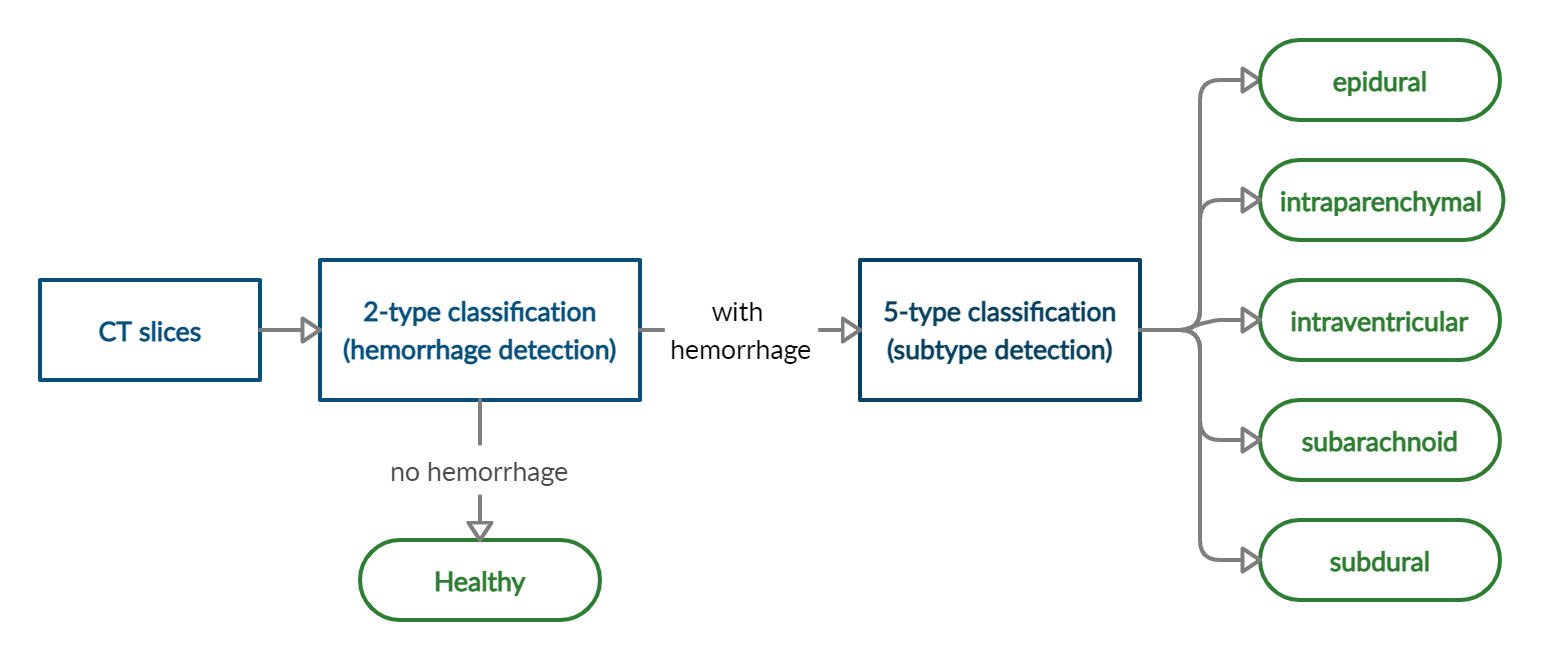
\includegraphics[width=14cm]{assets/images/mySolution.png}
\par\end{centering}
\caption{Diagram of the proposed solution \label{fig:solution}}
\end{figure}

In section 3.3, we discussed the topic of interpretable and explainable neural networks. In an attempt to make our model more trustworthy and eliminate the black-box issue, which deep learning models pose, we will make an effort to implement a Layer-wise Relevance Propagation algorithm. This algorithm could provide an explanation of how our neural network arrives at its predictions, since it produces a heatmap of those pixels, which contributed the most in the classification process.




\section{Our dataset}
In our work, we use a dataset provided by the Radiological Society of North America (RSNA)  \cite{RSNAchallenge}. The data was collected from four research institutions (Stanford University, Thomas Jefferson University, Unity Health Toronto and Universidade Federal de São Paulo) and put together for the RSNA Intracranial Hemorrhage Detection Challenge 2019, which was a competition held on the Kaggle platform\footnote{https://www.kaggle.com/c/rsna-intracranial-hemorrhage-detection/overview}. The dataset consists of training and testing set, which contain 752,803 and 121,232 individual CT slices respectively. 


A team of 60 radiology volunteers labeled the CT examinations according to the five intracranial hemorrhage subtypes - epidural (EPH), intraparenchymal (IPH), intraventricular (IVH), subarachnoid (SAH), subdural (SDH). Additional label named "any" is provided to indicate if any type of hemorrhage is present in the CT slice. Annotations are at disposal in a table format inside the corresponding csv file. All provided CT slices are in the DICOM (Digital Imaging and Communications in Medicine) format, which is the standard format for storing and transferring medical data. Along with the pixel data, this format also contains associated metadata, such as PatientID, StudyInstanceUID, SeriesInstanceUID and other. Even though the data is provided as individual CT scans, these can be grouped to form original CT scan by the ScanID, which can be found in the DICOM metadata. Each slice is a 16-bit grayscale image and has the spatial dimensions of 512x512 pixels. 
\begin{figure}[h]
\centering
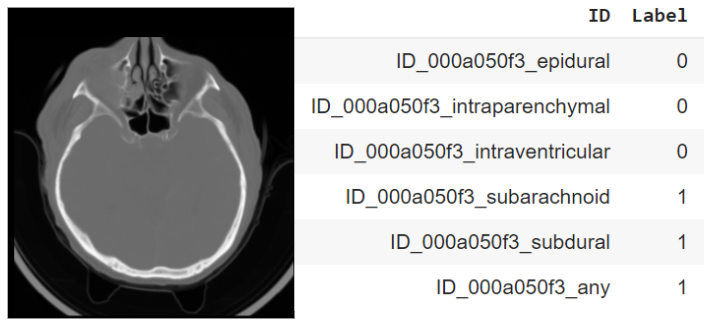
\includegraphics[width=10cm]{assets/images/datasetExample}
\caption{Example CT slice and corresponding annotation from the dataset \label{fig:dataset}}
\end{figure}

\section{Future work}
At present, we are working on the first stage of our proposed solution design. First experiments with a basic CNN architecture are being performed. The program is implemented in the Python language, using different deep learning and computer vision libraries. Due to a lack of accessible resources, our system is being developed on the Google Colab cloud platform, which offers access to faster GPUs and CPUs, making the training process more effective.


In the near future, we will work on gradually improving the performance of our model by different means. First of all, we will try different augmentation and pre-processing methods on our data. Inspired by the third presented related work \cite{relatedWork3}, we would apply different CT window settings to the slices, such as blood window, brain window or subdural window. This approach mimics the way radiologists work when analyzing a CT scan, therefore we believe it could help our CNN make better and more accurate predictions. The dataset we work with is relatively imbalanced, which could result in overfitting. Various image transformations such as image rotation, shifting or brightness changes could be applied in order to overcome this problem. After the first stage achieves satisfactory results, we will move on to implementation the slightly more challenging second stage, as well as the previously mentioned LRP algorithm, making our network interpretable and understandable.
